\chapter{Introduction}

\section{Research Background and Significance}
Reliable target understanding in complex dynamic scenes requires more than object detection in individual frames. A practical perception system must estimate where a target is, how it moves, whether it corresponds to an existing entity, and whether its behavior departs from normal scene evolution. These requirements are central to situation awareness, where low-level observations are converted into target states and higher-level scene interpretation \cite{endsley1995situation,blasch2009blueprint}. Target fusion and behavior analysis are therefore coupled tasks: behavior analysis depends on target states that are complete, consistent, and interpretable.

Single-modal sensing rarely satisfies these requirements in realistic environments. Optical images provide rich appearance, category, and contextual information, but they are sensitive to illumination, viewpoint, occlusion, weather, and missing geographic metadata. Electromagnetic and radar-like observations can provide complementary physical or motion-related cues, although they often carry weaker semantic information. Synthetic aperture radar (SAR) supports wide-area and all-weather observation, yet its imaging mechanism differs substantially from optical sensing. Existing trajectory records add temporal continuity and historical context, but they may be incomplete or inconsistent with newly observed targets. These complementary strengths motivate multimodal fusion rather than reliance on any single source.

Multimodal data become useful only after their cross-source relationships are made explicit. Different sensors may use different coordinate systems, sampling rates, spatial resolutions, and uncertainty models. They may also assign different identifiers to the same physical target. In some optical images, geographic coordinates may be unavailable. Target detections from these images then remain in the image plane and cannot directly enter a georeferenced trajectory system. If such observations are fused without reliable spatial and identity relationships, the resulting target states may contain false associations.

These limitations motivate the processing chain studied in this thesis. Coordinate-missing optical images are first connected to the trajectory system through visual reference retrieval and downstream target association. The resulting optical observations are then aligned with heterogeneous target entities through graph-based registration. The fused trajectories finally support individual and group behavior analysis. This design treats optical access, cross-modal fusion, and behavior analysis as connected stages rather than separate tasks. The following section formalizes this connected problem.

\section{Problem Description}
This thesis considers multimodal target fusion and behavior analysis under heterogeneous and partially incomplete observations. The available data include optical images with or without geographic metadata, target detections or modality-specific track fragments, electromagnetic observations, SAR observations, and existing target trajectories. These data sources provide complementary information, but they are not directly comparable. They may differ in spatial reference, temporal coverage, feature representation, and target identity assignment. The objective is to transform these heterogeneous observations into consistent entity-level target trajectories and then use the fused trajectories for behavior anomaly analysis and situation presentation.

A key sub-problem is the access of coordinate-missing optical images to the existing trajectory system. For coordinate-known optical images, detected targets can be represented in a common spatial frame and then considered by downstream target-association methods. For coordinate-missing optical images, however, target detections remain in the image plane and cannot be directly compared with georeferenced trajectories. Therefore, this thesis treats optical reference retrieval as a prerequisite for optical trajectory access. The retrieval result provides coordinate-known reference candidates and constrains the downstream target-level association process. It does not directly determine target identity or recover complete geographic trajectories.

Another sub-problem is entity-level registration across modalities. After single-modal preprocessing, each modality may produce its own target observations or trajectory fragments. These modality-specific target sets may contain the same physical targets, but their attributes, noise levels, sampling times, and confidence values can differ. The fusion problem is therefore not only to combine features, but also to estimate which entities from different modalities correspond to the same target. This thesis formulates the task as cross-modal entity registration, where target representations and relational structures are jointly used to estimate correspondences.

The final sub-problem is behavior analysis based on fused target trajectories. The fused trajectory is regarded as the target-level representation for subsequent analysis. Individual anomalies may appear as route deviation, abnormal speed, unusual trajectory shape, or sudden state change. Group-level anomalies may appear as inconsistent local motion, target departure from a group, group splitting, or group merging. The behavior analysis task is therefore defined as estimating interpretable anomaly indicators from both individual trajectories and group spatiotemporal relations.

Overall, the thesis addresses a connected problem chain. Coordinate-missing optical observations are first connected to the trajectory system through reference retrieval and target-level association constraints. Heterogeneous target entities are then aligned and fused. The fused trajectories are finally used for behavior analysis. This formulation separates the problem definition from the detailed technical challenges and provides the basis for the following chapters.

\section{Key Challenges}
The problem formulation above leads to several technical challenges. These challenges arise not only from the heterogeneity of the data sources, but also from the uncertainty that propagates across optical access, multimodal fusion, and behavior analysis.

Visual reference uncertainty is introduced by missing spatial metadata. Coordinate-missing optical images do not directly provide target locations in the same frame as existing trajectories. Their visual content may contain useful scene cues, but those cues can be distorted by viewpoint changes, illumination variation, seasonal appearance changes, occlusion, and dynamic objects. As illustrated in Fig.~\ref{fig:intro-vpr-challenges}, the same place may present different visual appearances across observation conditions. Training-based VPR also introduces an additional deployment burden because new scenes may lack labeled image pairs for training or domain adaptation. As a result, the system must establish reliable visual reference relationships under limited supervision and large appearance variation.

\begin{figure}[htbp]
  \centering
  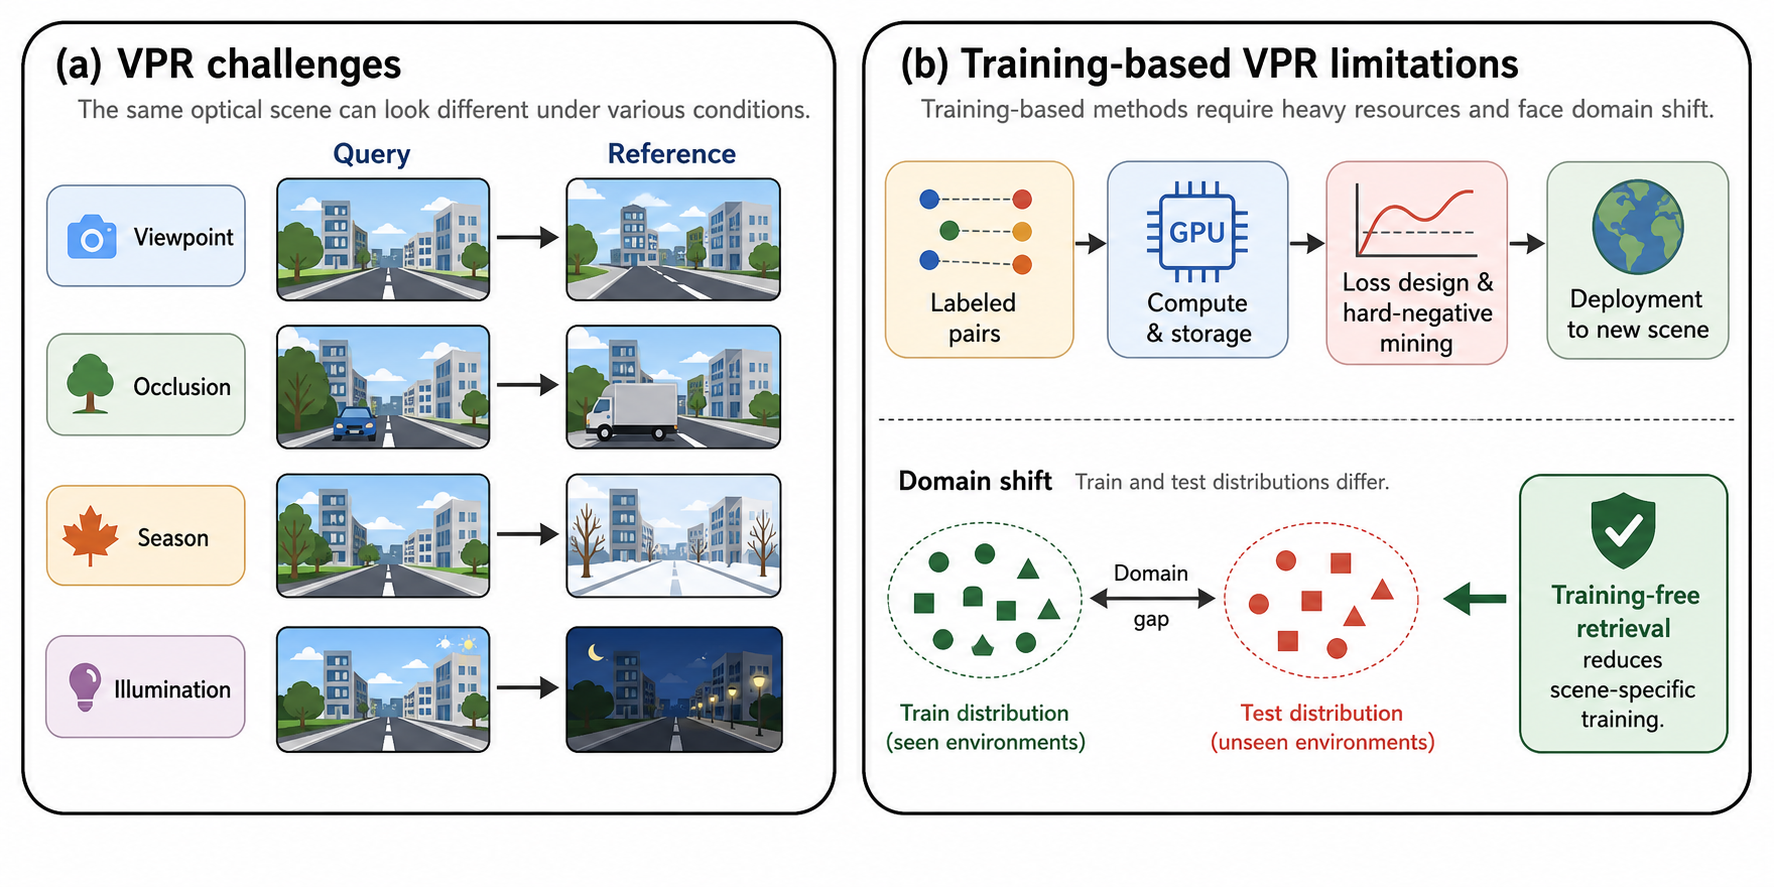
\includegraphics[width=0.95\linewidth]{images/chapter1/vpr_challenges_training_free_motivation.png}
  \caption{Conceptual illustration of VPR challenges and training-based VPR limitations in coordinate-missing optical scenes.}
  \label{fig:intro-vpr-challenges}
\end{figure}

Multimodal observation also introduces temporal inconsistency and incompleteness. This challenge is summarized in Fig.~\ref{fig:intro-temporal-inconsistency}, where optical, electromagnetic, and SAR observations are shown as separate timelines rather than naturally aligned frames. The colored windows indicate intervals in which a modality can provide observations, while the markers and gray crosses distinguish valid observations from missing ones at the reference times. The figure therefore makes two sources of incompleteness explicit. First, temporal incompleteness arises because sensors have different sampling rates and may produce interrupted tracklets. Second, spatial incompleteness arises because the sensor footprints or fields of view may not cover the same region at the same time. As a result, a target can be observed in one modality while absent in another, and a reference time may contain only partial or asynchronous evidence. Direct frame-level fusion is unstable under this condition because a complete synchronized multimodal observation tuple cannot be assumed. The fusion representation must instead tolerate missing observations, align asynchronous tracklets, and account for modality-dependent reliability.

\begin{figure}[H]
  \centering
  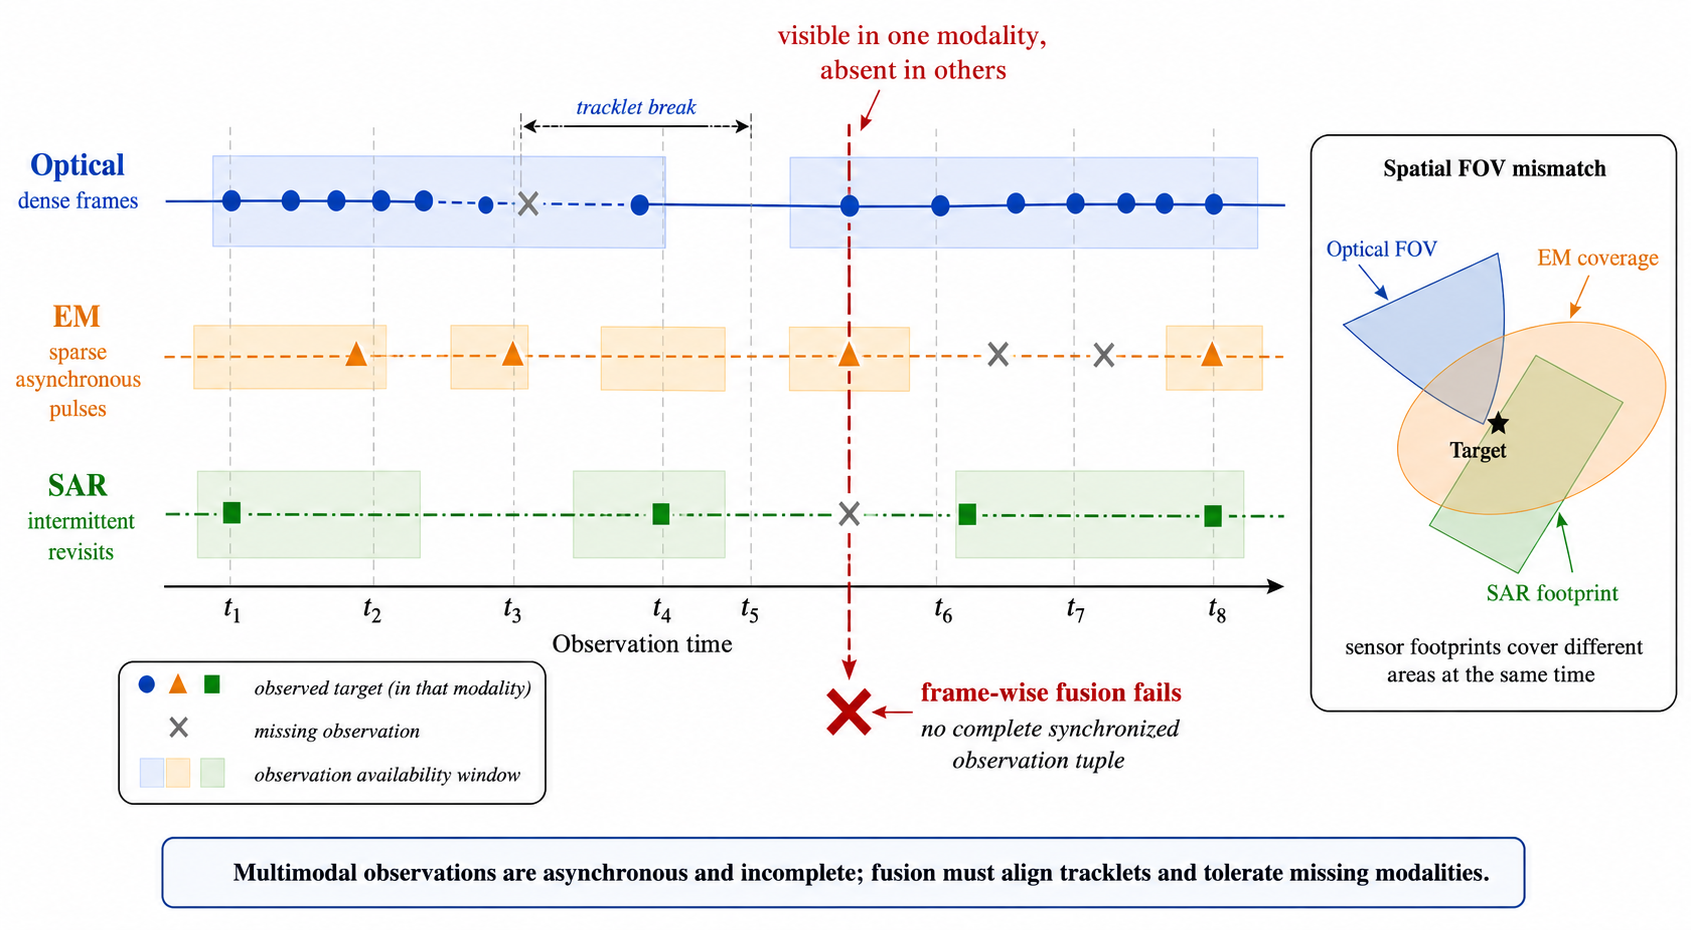
\includegraphics[width=0.95\linewidth]{images/chapter1/temporal_inconsistency_incomplete_observation.png}
  \caption{Temporal inconsistency and incompleteness in multimodal observation. The figure shows why asynchronous sampling, interrupted observations, and spatial coverage mismatch make direct frame-level fusion unreliable.}
  \label{fig:intro-temporal-inconsistency}
\end{figure}

Cross-modal identity ambiguity further arises from heterogeneous representations. As illustrated in Fig.~\ref{fig:intro-cross-modal-identity}, each modality may form its own target graph with modality-specific node attributes, missing entities, and neighborhood relations. Optical observations mainly provide appearance and semantic cues, electromagnetic observations describe signal-related responses, and SAR observations capture scattering and spatial response patterns. These heterogeneous representations create two coupled difficulties. First, different targets within one modality may have similar local features, such as visually similar optical targets. Second, the same physical target may appear dissimilar across modalities because its optical appearance, electromagnetic signal, and SAR response are generated by different sensing mechanisms. The local similarity matrices in Fig.~\ref{fig:intro-cross-modal-identity} show the resulting ambiguity: a feature-only matcher may produce multiple high-score candidate correspondences, such as several optical targets competing for one electromagnetic target or one electromagnetic target being compatible with multiple SAR detections. Therefore, cross-modal association cannot rely only on local feature similarity. It must be treated as a graph-level assignment problem that jointly exploits temporal continuity, spatial compatibility, and relational structure among targets.

\begin{figure}[H]
  \centering
  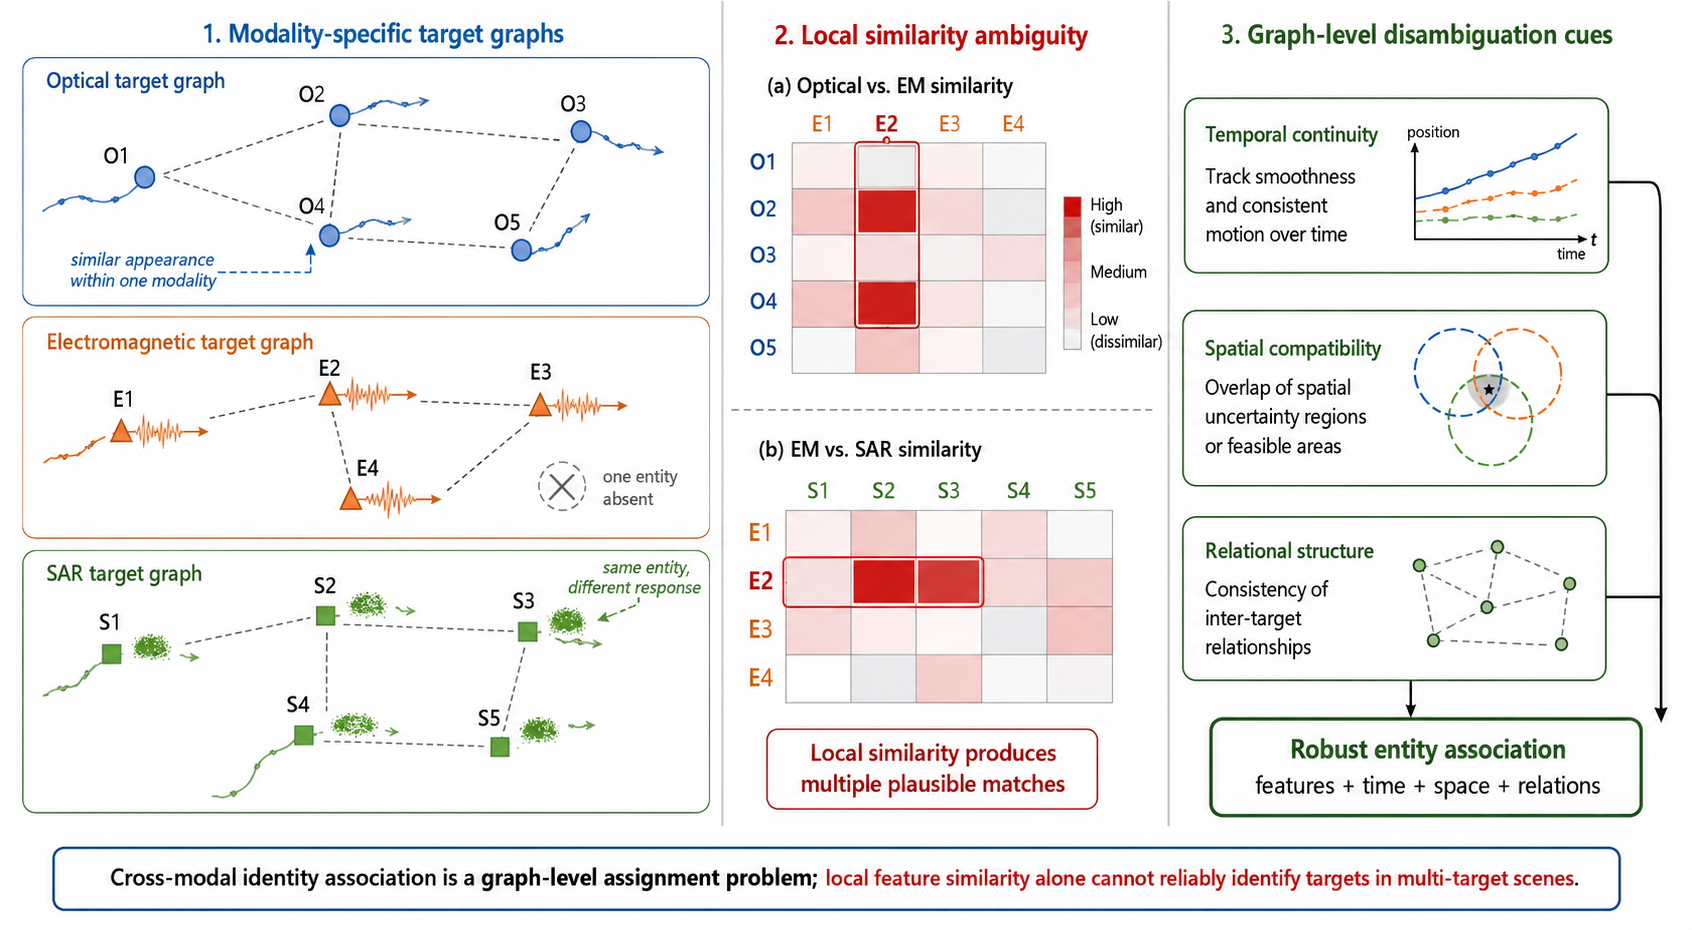
\includegraphics[width=0.98\linewidth]{images/chapter1/cross_modal_identity_ambiguity.png}
  \caption{Cross-modal identity ambiguity under heterogeneous target representations. The figure shows that local feature similarity can produce multiple plausible matches, so identity association must also use temporal, spatial, and relational consistency.}
  \label{fig:intro-cross-modal-identity}
\end{figure}

Behavior analysis must remain interpretable under fused-data uncertainty. As shown in Fig.~\ref{fig:intro-behavior-uncertainty}, the behavior analysis stage receives fused trajectories rather than ground-truth motion traces. These trajectories may still contain localization uncertainty, missing observations, cross-modal association errors, and noisy fused states caused by the previous optical access and multimodal fusion stages. The middle part of the figure separates behavioral evidence into two levels. Individual-level evidence describes route deviation, abnormal speed, and unusual motion shape, while group-level evidence describes relative motion changes, neighborhood structure variation, and membership changes. These two levels do not always agree. A trajectory may look normal in isolation but abnormal relative to its group. Conversely, a short individual anomaly may not indicate a meaningful situation-level event if the group relation remains stable. Therefore, the output should not be limited to a single anomaly score. It should combine uncertainty-aware score curves, explanation tags, and spatial event summaries so that the system can indicate both what is abnormal and how reliable the supporting evidence is. The behavior analysis method must therefore provide anomaly indicators that are robust to upstream uncertainty and interpretable for situation assessment.

\begin{figure}[H]
  \centering
  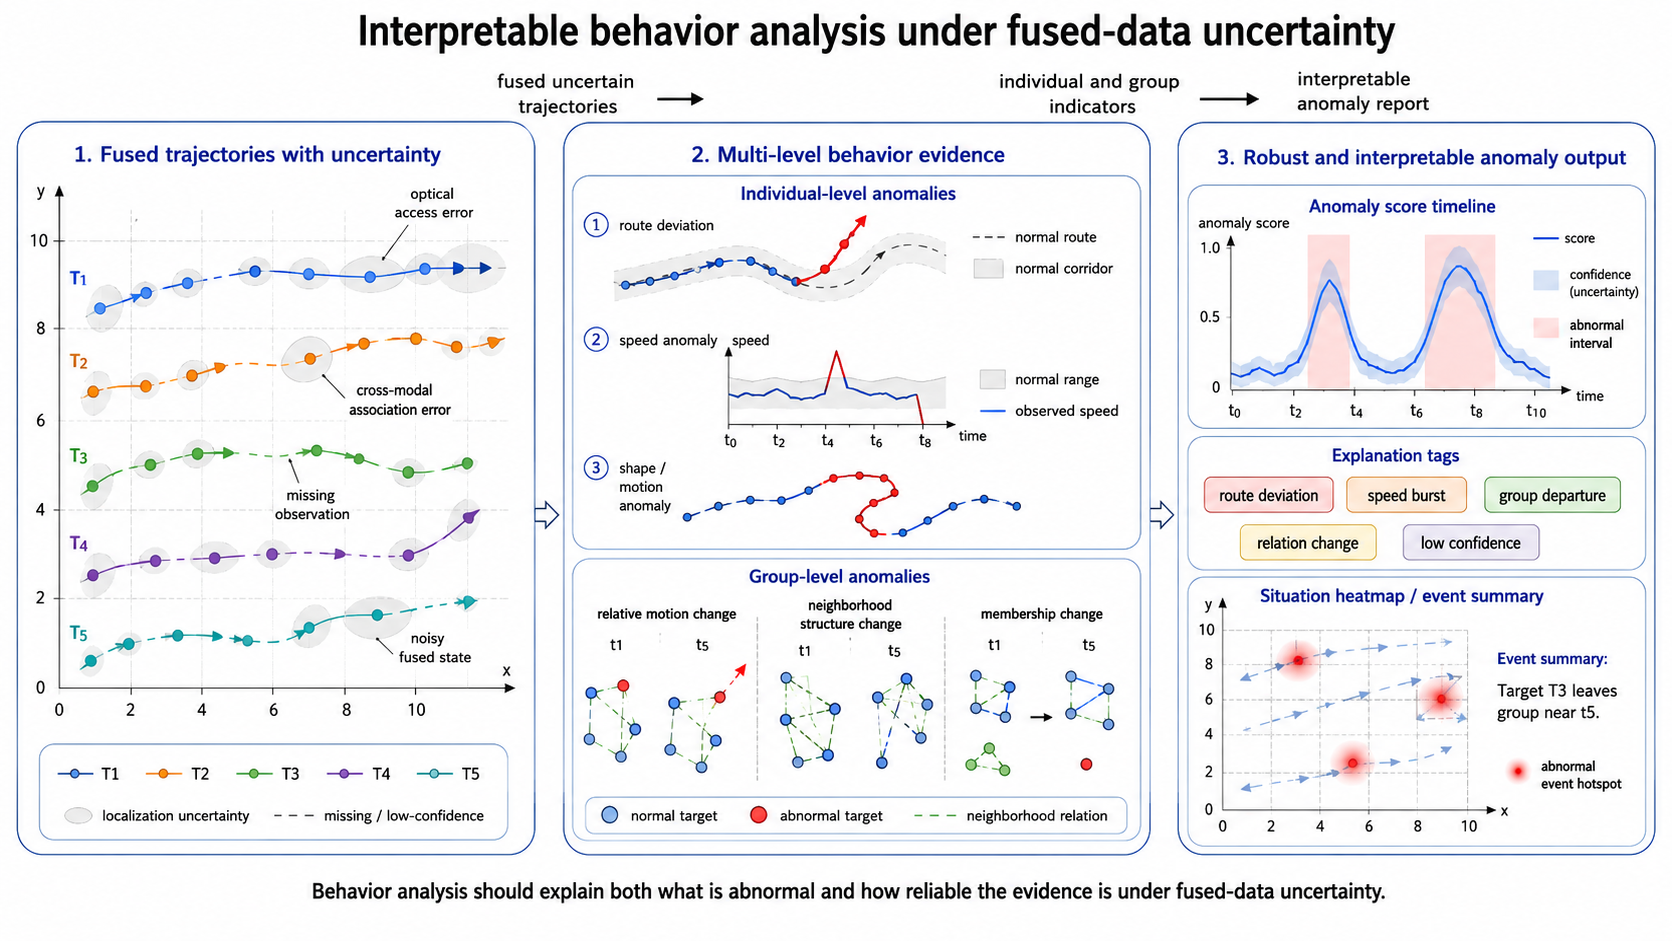
\includegraphics[width=0.98\linewidth]{images/chapter1/interpretable_behavior_uncertainty.png}
  \caption{Interpretable behavior analysis under fused-data uncertainty. The figure links uncertain fused trajectories to individual and group anomaly evidence, highlighting that the output should explain both abnormal behavior and evidence reliability.}
  \label{fig:intro-behavior-uncertainty}
\end{figure}

These challenges motivate a review of related work on visual place recognition, multimodal target fusion, graph-based registration, and trajectory-based anomaly detection.

\section{Related Work}

\subsection{Visual Place Recognition and Optical Trajectory Association}
Visual place recognition (VPR) aims to retrieve reference images that depict the same or a nearby physical location as a query image \cite{yin2025gprs,wang2026tfvpr}. It is a core component in robotic localization, loop-closure detection, long-term navigation, and visual retrieval \cite{murartal2017orbslam2,milford2008seqslam}. In this thesis, VPR is introduced for a narrower purpose. It supports coordinate-missing optical access by providing scene-level reference candidates, rather than by making target-level identity decisions.

The main difficulty in VPR is appearance variation. The same place may differ substantially across viewpoints, illumination conditions, seasons, occlusions, and domains \cite{yin2025gprs,wang2026tfvpr}. As shown in Fig.~\ref{fig:intro-vpr-challenges}, this difficulty is especially relevant to coordinate-missing optical images, because visual content is the only available cue for establishing a reference relationship with coordinate-known scenes.

Existing VPR methods have developed from hand-crafted retrieval pipelines to learned visual descriptors. Early systems often used local feature aggregation strategies such as Bag-of-Words and VLAD \cite{galvez2012bags,jegou2010vlad}. Deep VPR methods then improved descriptor discriminability through several complementary routes, including trainable VLAD-like aggregation, local-to-global patch matching, geographically structured supervision, viewpoint-robust training, and holistic feature mixing \cite{arandjelovic2016netvlad,hausler2021patchnetvlad,berton2022cosplace,berton2023eigenplaces,alibey2023mixvpr}. Graph-based VPR methods further exploit relationships among regions or patches to improve robustness under viewpoint changes and local ambiguity \cite{qin2021gatvpr,zuo2025prgs,chen2025sage}.

Despite these advances, many high-performing VPR methods still depend on scene-level supervision signals, such as paired place images, geographic labels, task-specific training objectives, or target-domain optimization \cite{arandjelovic2016netvlad,berton2022cosplace,alibey2023mixvpr}. These requirements limit their use when a new scene lacks reliable annotations. Large-scale visual pretraining provides a more flexible alternative: contrastive image-text learning, vision transformers, masked image modeling, and self-supervised dense representation learning have all shown the ability to produce transferable visual features \cite{radford2021clip,dosovitskiy2020vit,he2022mae,oquab2023dinov2}. AnyLoc shows that frozen foundation-model features can support zero-shot place recognition \cite{keetha2024anyloc}, while TF-VPR further studies training-free descriptor generation and refinement for VPR \cite{wang2026tfvpr}. This training-free direction matches the setting of this thesis. It reduces dependence on scene-specific annotation and provides coordinate-known reference candidates for downstream optical trajectory association. The detailed method is presented in Chapter 3.

\subsection{Multimodal Target Fusion}
Multimodal target fusion seeks to combine heterogeneous observations into target states that are more complete and reliable than those from a single sensor. Multisensor fusion research commonly distinguishes signal-level fusion, object-level estimation, and situation-level interpretation \cite{hall1997multisensor,blasch2009blueprint}. In target analysis, this hierarchy is often reflected in feature-level, decision-level, and target-level fusion.

Feature-level fusion projects heterogeneous observations into a shared representation before prediction or association. It can exploit complementary information at an early stage, but it usually assumes accurate temporal and spatial alignment. Decision-level fusion combines outputs from modality-specific models. This strategy is easier to deploy when sensors have separate processing pipelines, but it may lose fine-grained target interactions. Target-level fusion focuses on whether observations correspond to the same physical entity and how their states should be integrated. This level is most relevant to this thesis because behavior analysis requires consistent trajectories, not independent modality-specific decisions.

The central limitation of practical target-level fusion is that heterogeneous observations are rarely aligned in advance. Different modalities may have different sampling rates, localization accuracy, attribute spaces, and missing-observation patterns. Recent studies on multimodal registration and fusion show that cross-source alignment must account for geometry, semantics, uncertainty, and modality-specific reliability \cite{wu2024jointsemantic,chen2026multimodal,zhang2025optsar}. These requirements connect multimodal fusion to entity correspondence estimation. Graph modeling and registration therefore provide a more specific technical route for the present work.

\subsection{Graph Modeling and Entity-Level Registration}
Graph modeling provides a structured way to represent targets and their relations. A graph can encode target attributes as node features and describe temporal continuity, spatial neighborhoods, or contextual dependencies as edges. This representation is useful in multi-target scenes because identity consistency often depends on both local target evidence and relational structure.

Single-modal tracking methods provide an important basis for target identity maintenance. Classical probabilistic methods, including multiple hypothesis tracking and joint probabilistic data association, model uncertainty under missed detections and clutter \cite{reid1979mht,fortmann1983jpda}. Modern tracking-by-detection methods maintain trajectory continuity by combining efficient motion prediction, deep appearance association, low-confidence detection recovery, and robust association strategies such as camera-motion compensation \cite{bewley2016sort,wojke2017deepsort,zhang2022bytetrack,aharon2022botsort}. These methods are effective for producing modality-specific trajectories. However, they do not by themselves resolve correspondence between entities observed by different modalities.

Graph matching and registration extend this idea from within-modality association to cross-set alignment. Instead of matching isolated nodes independently, graph matching seeks correspondences supported by both node similarity and structural consistency. This property is valuable when local target features are ambiguous but relational roles remain informative. Registration methods have developed from iterative closest point and its variants \cite{besl1992icp,rusinkiewicz2001icpvariants,segal2009gicp} to probabilistic, soft-assignment, and learning-based correspondence estimation \cite{gold1996softassign,myronenko2010cpd,wang2019dcp,yew2020rpmnet}. Recent graph-based registration studies further improve robustness under structural ambiguity and incomplete observations \cite{fu2023deepgraphmatching,zhao2022graphreg,liu2024s2anet}.

These studies suggest that multimodal entity registration should use both attributes and relations. The same physical target may appear different across modalities, whereas its motion trend, temporal continuity, and relation to neighboring targets may remain more stable. This thesis therefore uses graph-based entity registration as the main route for cross-modal target alignment. Chapter 4 details the trajectory encoding, graph interaction, soft correspondence estimation, and fusion strategy.

\subsection{Research on Behavior Analysis and Anomaly Detection}
Trajectory-based behavior analysis studies how motion traces reflect normal movement, abnormal deviation, and higher-level target activity. Classical trajectory mining methods use geometric similarity, density statistics, clustering, and local segmentation. TRACLUS partitions trajectories into line segments and groups similar sub-trajectories to identify common movement patterns \cite{lee2007traclus}. Partition-and-detect methods show that abnormality may occur in a local trajectory segment rather than in the full track \cite{lee2008traod}. Isolation-based methods identify unusual trajectories by measuring how easily they can be separated from normal patterns \cite{zhang2011ibat}.

Recent trajectory anomaly detection has shifted toward learned normal-pattern modeling. Current methods study route, speed, and shape anomalies, diffusion-based reconstruction, context-aware scoring, and graph-enhanced trajectory anomaly detection \cite{cao2025cetrajectory,li2024difftad,hu2024contexttrajad,mbuya2025getad}. These studies indicate that abnormal behavior should be analyzed from multiple aspects of a trajectory rather than through a single distance measure.

Individual trajectory analysis is not sufficient when behavior is constrained by neighboring targets. Multi-agent prediction research has shown that such dependencies can be modeled through social pooling, adversarial generation of socially plausible futures, spatiotemporal graph convolution, graph-structured recurrent forecasting, and agent-aware attention \cite{alahi2016sociallstm,gupta2018socialgan,mohamed2020socialstgcnn,salzmann2020trajectronpp,yuan2021agentformer}. For anomaly detection, this implies that a target may be abnormal because its relation to a group changes, even when its individual trajectory appears plausible.

Spatiotemporal graph anomaly detection provides mechanisms for this relational analysis. Recent methods explicitly model feature-wise and temporal dependencies, learn inter-sensor graph structures, capture intra- and inter-modal correlations, and handle missing or irregularly sampled observations through graph-based temporal processes \cite{zhao2020mtadgat,deng2021gdn,ding2023mstgat,zheng2024gstpro}. Situation presentation further requires mapping anomaly scores into interpretable spatial outputs. Kernel density estimation and spatiotemporal hotspot mapping provide common tools for this purpose \cite{hu2018stkde,han2023cstkde,jing2024sthgnet,shao2025tnkde}. Based on these ideas, this thesis analyzes behavior from fused target trajectories rather than raw video actions. Chapter 5 presents individual anomaly scoring, group consistency analysis, and heatmap generation.

\section{Research Content and Contributions}

\subsection{Research Content}
The research content of this thesis is organized around a connected processing route from multimodal observations to situation-level behavior output. As shown in Fig.~\ref{fig:intro-technical-route}, the route first constructs modality-specific trajectories from heterogeneous inputs, then performs entity-level multimodal registration and reliability-aware fusion, and finally analyzes individual behavior, group behavior, and regional situation patterns. The figure also shows how the main technical stages correspond to the following chapters.

\begin{figure}[H]
  \centering
  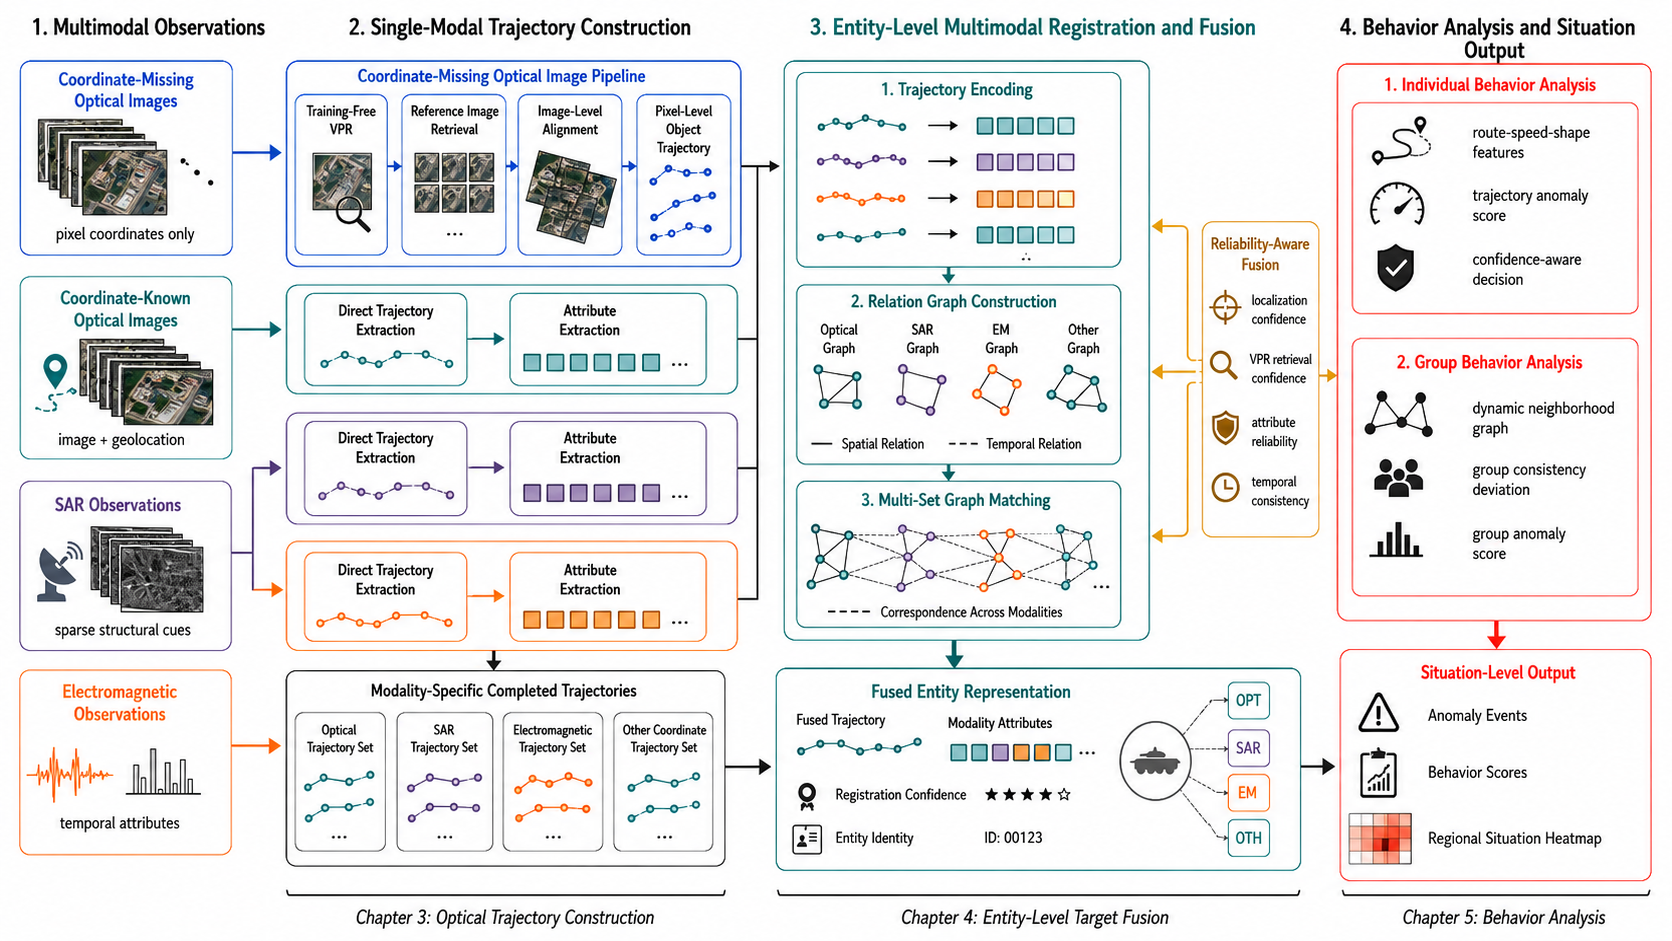
\includegraphics[width=\linewidth]{images/chapter1/overall_technical_route.png}
  \caption{Overall technical route of the proposed multimodal target fusion and behavior analysis system. The pipeline links multimodal observations, single-modal trajectory construction, entity-level registration and fusion, and behavior analysis with situation-level output.}
  \label{fig:intro-technical-route}
\end{figure}

First, corresponding to the single-modal trajectory construction stage in Fig.~\ref{fig:intro-technical-route}, this thesis addresses optical reference retrieval for coordinate-missing images. When reliable geographic coordinates are unavailable, pixel-level target detections cannot be directly transformed into the coordinate frame of existing trajectories. To provide a scene-level access mechanism, this thesis introduces a training-free VPR module based on TF-VPR. The module retrieves coordinate-known reference images for a coordinate-missing query and produces ranked visual reference candidates. These candidates do not serve as direct target-identity decisions; instead, they constrain downstream target association and support optical trajectory access.

Second, corresponding to the entity-level registration and fusion stage in Fig.~\ref{fig:intro-technical-route}, this thesis investigates multimodal target fusion through entity-level registration. After optical observations are connected to the trajectory system, they need to be fused with electromagnetic, SAR, and historical trajectory information. This stage formulates fusion as a cross-modal entity registration problem. Modality-specific trajectories are encoded as target-level representations, graph interaction refines these representations using intra-set structure and cross-set information, and a soft correspondence matrix estimates entity alignments across modalities. The aligned observations are then integrated into unified target trajectories.

Third, corresponding to the behavior analysis and situation output stage in Fig.~\ref{fig:intro-technical-route}, this thesis develops behavior analysis methods for fused multimodal target data. The fused trajectories are used as target-level inputs for individual and group behavior analysis. Individual analysis characterizes route, speed, and shape deviations, whereas group analysis characterizes spatiotemporal consistency, neighborhood variation, splitting, merging, and other relational changes. The outputs include anomaly scores, interpretable event labels, and situation heatmaps.

\subsection{Contributions}
The main contributions of this thesis are summarized as follows.

\begin{enumerate}
  \item This thesis constructs an integrated framework for multimodal target fusion and behavior analysis. The framework links coordinate-missing optical access, cross-modal entity registration, target-level fusion, and behavior anomaly analysis, thereby clarifying the input-output relationships among the main modules and supporting system-level implementation.

  \item This thesis introduces a TF-VPR-based optical reference retrieval strategy for coordinate-missing optical images. The strategy retrieves coordinate-known reference images without additional training on the target scene and uses the resulting candidates to constrain downstream target-level association, thereby reducing dependence on labeled place-recognition data in new scenes.

  \item This thesis designs an entity-level multimodal fusion method based on trajectory representation and graph matching. The method represents modality-specific trajectories as structured entity sets, refines their features through intra-set and cross-set interactions, estimates soft correspondences, and fuses matched observations into unified target trajectories.

  \item This thesis develops a behavior analysis method driven by fused trajectories. The method combines individual anomaly indicators with group-level spatiotemporal consistency analysis, supporting anomaly detection from both single-target motion patterns and multi-target relational changes.
\end{enumerate}

\section{Organization of the Thesis}
The remainder of this thesis is organized as follows.

Chapter 2 presents the overall system architecture and multimodal data modeling. It defines the input data sources, preprocessing flow, unified target representation, and module roles.

Chapter 3 studies optical reference retrieval with TF-VPR. It focuses on coordinate-missing optical images, training-free visual place recognition, and the use of retrieval results for downstream target association.

Chapter 4 studies multimodal target fusion and entity-level registration. It describes trajectory encoding, graph interaction, soft matching, cross-modal correspondence estimation, and entity-level fusion.

Chapter 5 studies behavior analysis based on fused multimodal data. It introduces individual trajectory anomaly scoring, group spatiotemporal consistency analysis, event interpretation, and situation heatmap generation.

Chapter 6 presents system implementation and integrated demonstration. It describes the implementation environment, major modules, data flow, and demonstration workflow.

Chapter 7 concludes the thesis. It summarizes the main research work, discusses limitations, and outlines future directions.
